\label{sec:training-data}

This section describes the synthetic corpus used for mid-training of our context-grounded QA model. The corpus is built to exercise the three properties stated in Section~\ref{sec:model-design-principles}: requires reasoning over the supplied context; every answer is recoverable from the context alone to avoid memorization; and a fraction of examples carry insufficient evidence, so abstention becomes a learned response. Each training instance consists of a question, one or more golden context chunks from Wikipedia containing all supporting facts, semantically similar distractor contexts, a structured reasoning trace, and the final answer (or ``Not enough information'' for refusal cases).

The corpus is built as a mix of three subsets of increasing difficulty, covering a broad range of questions from simple single-hop lookups to complex multi-hop fusions. Easier examples (single-hop lookup) are cheap and abundant; harder ones (multi-hop fusion) are progressively more expensive to generate cleanly, and their volume is correspondingly smaller, see Section~\ref{sec:synth-sh-analysis}. 

\subsection{Single-Hop QA Generation}
\label{sec:synth-singlehop}
Single-hop questions are those that can be answered using information from a single paragraph, without requiring multi-step reasoning, aggregation, or arithmetic operations. This category represents the largest portion of the dataset, as high-quality single-hop examples are relatively inexpensive to generate at scale, and because relevance filtering remains the primary challenge in real-world deployment.

The pipeline for single-hop QA generation has four stages: ingest and chunk page, generate QA, mine distractors, and filter. We describe each in turn.

\begin{enumerate}
    \item \textbf{Ingesting and chunking} \hspace{0.5em} In the English Wikipedia XML dump, each page is run through a wikitext cleaner that strips templates, references, infoboxes, and gallery markup. A page is split into paragraphs, and each paragraph becomes a candidate \textit{chunk}. A chunk is precisely the unit of context the trained model sees.
    \item \textbf{QA Generation} \hspace{0.5em} For each gold paragraph, we issue a single call to \texttt{gpt-oss-120B}~\citep{openai2025gptoss120bgptoss20bmodel}, asking for ten short QA pairs returned as a JSON array. It instructs the LLM that questions must be self-contained and answers must be short and extractive.
    \item \textbf{Distractor mining} \hspace{0.5em} For every gold page, we fetch up to one thousand child pages from the Wikipedia link graph and apply the same cleaning and chunking routine as described earlier. Every resulting child paragraph is scored against the gold paragraph by TF-IDF cosine similarity. We keep the top twenty children by similarity.
    \item \textbf{Filtration} \hspace{0.5em} In the final stage, an LLM-as-judge evaluates the generated QA pairs. This step filters out any pairs that are inaccurate or lack logical flow, ensuring only high-quality data remains. Detailed criteria are provided in Section~\ref{sec:synth-traces}.
\end{enumerate}

\subsection{Multi-hop QA Generation}
\label{sec:synth-multihop}

Multi-hop QA questions require the synthesis of multiple facts rather than simple span extraction from a single sentence. To ensure that questions remain strictly grounded in the provided evidence, we condition its generation on a knowledge graph (KG) extracted from the context (gold and distractor chunks), requiring the LLM to follow an explicit reasoning path sampled from the KG. We employ this KG-conditioned pipeline to address three fundamental limitations that arise when attempting to generate multi-hop questions using the same approach as for single-hop QA:

\begin{itemize}
    \item  \textbf{Lack of structural support} \hspace{0.5em} Many passages contain sufficient fact density for single-hop questions but lack the ``bridge'' entities necessary for multi-hop reasoning. Our approach resolves this by sampling reasoning paths directly from the KG, which guarantees the existence of such bridges.
    \item  \textbf{Verification complexity} \hspace{0.5em} Questions that are complex to answer are often equally difficult to verify, as a generated question may be valid while the LLM's answer to it is not. By conditioning generation on a specific path, the gold answer is fixed by the path itself rather than being subject to the generator’s output.
    \item  \textbf{Lack of structural control} \hspace{0.5em} Free-form generation often results in questions with unknown reasoning structures, making it impossible to analyze or balance the corpus by question type. In contrast, sampling chains from the KG provides full control over the structural and compositional complexity of the generated dataset.
\end{itemize}    

\subsubsection{Knowledge Graph Extraction}
We extract gold paragraphs and their associated distractors from the training split of the MuSiQue~\citep{musique} dataset. To achieve fine-grained control over automatic question generation, we employ the Knowledge Graph (KG) extraction pipeline introduced in Wikontic~\citep{chepurova-etal-2026-wikontic}. This pipeline transforms unstructured text into a structured factual graph, which serves as the backbone for our controlled multi-hop QA generation. Wikontic employs ontological constraints from Wikidata to eliminate redundant and inconsistent information and performs entity normalization and de-duplication to maximize graph connectivity.   We utilize \texttt{gpt-oss-120b}~\citep{openai2025gptoss120bgptoss20bmodel} as the base model for Wikontic.

The extracted KGs are then stored in an RDF database, facilitating efficient structural queries and subgraph retrieval. This representation allows us to explicitly select subgraphs based on predefined topological properties such as path length, branching factor, and relation types, providing precise control over the reasoning complexity of our generated multi-hop questions.

\subsubsection{Path Sampling and Question Types}
To control the complexity of the generated data, we adopt the question taxonomy of the DRAGOn benchmark~\citep{dragon}. Specifically, we generate \emph{simple} questions, three families of two-hop questions (\emph{set}, \emph{multi-hop}, and \emph{condition}), and three-hop \emph{bamboo}-style questions. Each type corresponds to a separate SPARQL template that selects a sub-graph of a given shape and rejects degenerate cases via additional filters. 

For every sampled path the LLM receives a short, type-specific prompt that specifies (1) the reasoning structure, (2) the gold path, (3) the supporting paragraphs, and (4) hard requirements on the output: the question must be self-contained, the answer must be a literal span of the supplied context, and the answer must be reachable only by following the path. For every sampled path we issue a single call to \texttt{gpt-oss-120B} with the type-specific prompt to generate a QA pair.

\subsubsection{Unanswerable Question Construction}
\label{sec:unans}

A fraction of our corpus includes refusal examples, where the model should abstain when the provided evidence is insufficient. 
To generate these ``hard'' refusal cases, we use a DeBERTa model fine-tuned on SQuAD~\citep{deeppavlov1} to answer questions using reduced subsets of the original gold contexts. If the predicted answer does not match the original one, the model should abstain. The intuition is that if a strong extractive model cannot recover the answer, a critical piece of information is missing, even though relevant evidence remains in the context.

\begin{figure}[H]
\centering
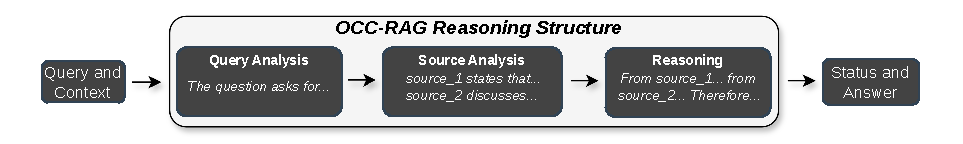
\includegraphics[width=\textwidth]{images/youtu_noemoji.pdf}
\caption{Structure of OCC-RAG output. The model proceeds through three named sections: \emph{Query Analysis} identifies what the question asks and the entities involved, \emph{Source Analysis} attributes relevant facts to specific source passages, and \emph{Reasoning} combines them to derive the answer. This structure keeps every conclusion tied to the supplied context and yields a calibrated \texttt{ANSWERABLE}/\texttt{UNANSWERABLE} status alongside the final answer.}
\label{fig:occ-output}
\end{figure}

\subsection{Structured Reasoning}
\label{sec:synth-traces}

To make the three target behaviours of Section~\ref{sec:model-design-principles} (multi-hop inference, evidence grounding, and calibrated abstention) learnable from token-level supervision rather than left implicit, we enrich every QA pair in the corpus with an explicit reasoning trace. The trace structure is illustrated in Figure~\ref{fig:occ-output} and described in detail below; a sample of the prompt/response format can be found in Figure~\ref{fig:trace-training-example} (Appendix~\ref{sec:prompt-trace}).

\paragraph{Reasoning Format}
We adopt the trace format of Pleias-RAG~\citep{pleias}, in which the reasoning is laid out as a sequence of named sections. The first section, \emph{Query Analysis}, describes what the question asks and which entities and relations are involved. The second, \emph{Source Analysis}, identifies which of the supplied sources are relevant and what each one contributes. The third, \emph{Reasoning}, shows how the relevant facts are combined into the final answer. A closing \emph{Answer} section carries the answer string. To this scaffold we add a \emph{Status} section that emits an explicit \texttt{ANSWERABLE}/\texttt{UNANSWERABLE} verdict immediately before the final answer. The addition is motivated by our refusal objective: turning abstention into a discrete label that the model has to commit to before producing the answer makes the decision boundary between answerable and unanswerable cases an explicit supervised target, rather than something the model has to infer from the wording of the answer alone.

\paragraph{Generation}
We generate reasoning traces using \texttt{Qwen3.5-27B}. For sampling parameters we use the values recommended in the original model card\footnote{\url{https://hf.co/Qwen/Qwen3.5-27B}}. We disable thinking mode during generation for two reasons. First, enabling Qwen's native thinking adds substantial generation cost, as the model emits an additional internal trace before producing the structured output. Second, on our development slice, this extra native reasoning did not yield a meaningful improvement in distilled-student quality. We emphasize that this concerns only the model's built-in thinking mode, as the structured reasoning trace emitted in our own format (described above) is exactly the supervision signal we want the student to learn and is always present in every generation. \texttt{Qwen3.5-27B} was itself selected over other open-weight generators by distilled-student performance on a held-out development slice covering every question type and both answerable and refusal cases.

\paragraph{Filtering}
Each generated trace passes through four checks. (1) \emph{Format}: we check that all the fields (Query Analysis, Source Analysis, Reasoning, Status, Answer) are preserved; traces with a missing section are dropped. (2) \emph{Answer match}: the predicted answer is compared to the gold answer by exact match; on answerable examples, a mismatch causes the trace to be dropped, and on refusal examples, any trace that asserts a non-refusal answer is dropped as well. (3) \emph{LLM-as-a-judge}: examples that fail exact match are then re-checked by \texttt{Qwen3-4B}, prompted as a verifier, which compares the predicted answer against the gold; traces the judge does not endorse are dropped. (4) \emph{Overthinking}: as noted above, \texttt{Qwen3.5-27B} is prone to overthinking, producing long reasoning chains on questions that admit a short solution. We filter these in two stages. First, we drop any trace whose reasoning section exceeds $1{,}256$ tokens. Second, we drop any trace containing more than ten \emph{thinking markers} such as \texttt{Wait} and \texttt{Alternatively} which we collected manually by inspecting the long tail of the trace-length distribution. 

\subsection{Dataset Statistics}
\label{sec:synth-sh-analysis}

The final corpus contains approximately 3.25M QA pairs, which include 2.78M single-hop pairs, 262k multi-hop single-context pairs answered within a single passage, 165k multi-hop multi-context pairs requiring cross-passage information fusion, and 43k abstain pairs where no passage supports the answer. In total, the dataset encompasses roughly 8B Qwen3-tokens, where the single-hop subset dominates the overall budget (7.76B tokens). Across the corpus, distractor contexts consume the largest share of tokens (35\%--75\%), followed by gold contexts and reasoning chains, see Figure~\ref{fig:token_budget}. 

   % distractor series fill and draw

\begin{figure}[htbp]
    \centering
    \resizebox{\linewidth}{!}{%
    \begin{tikzpicture}
        \definecolor{airigreen}{HTML}{A8E6CF}
        \definecolor{airigreendark}{HTML}{7BC8A4}        
        \definecolor{emerald}{HTML}{50C878}
        \definecolor{color1}{HTML}{FFEF91}
        \definecolor{color2}{HTML}{FFA02E}
        \begin{groupplot}[
            group style={
                group size=2 by 1,
                horizontal sep=2cm,
            },
            width=7cm,
            height=5cm,
            y=1cm,
            enlarge y limits=0.25,
            xmin=0,
            tick label style={font=\footnotesize},
            tick label style={font=\scriptsize},
            label style={font=\small},
            title style={font=\small\bfseries},
            axis lines*=left,
            axis line style={black!70},
            legend style={font=\footnotesize, draw=none, fill=none},
        ]
        % ================= LEFT PLOT: TOTAL TOKENS =================
        \nextgroupplot[
            xbar,
            bar width=0.4cm,
            xmode=linear,
            title={Total tokens},
            xlabel={Tokens},
            xtick={0,1,2,3},
            xticklabels={0.01B,0.1B,1B,10B},
            xmin=0,xmax=3.8,
            symbolic y coords={Abstain,{MH single},{MH multi},{Single-hop}},
            ytick=data,
            nodes near coords,
            every node near coord/.append style={anchor=west, font=\scriptsize},
            point meta=explicit symbolic,
        ]
        % Coordinates mapped to log10 scale + 2 to force bars from 0
        \addplot[fill=airigreen, draw=airigreendark] coordinates {
            (2.8899,{Single-hop}) [7.76B]
            (1.3222,{MH multi}) [0.21B]
            (1.2041,{MH single}) [0.16B]
            (0.4624,Abstain) [0.029B]
        };
        % ================= RIGHT PLOT: COMPOSITION =================
        \nextgroupplot[
            xbar stacked,
            bar width=0.4cm,
            title={Composition},
            xlabel={Share of subset tokens},
            xtick={0,25,50,75,100},
            xticklabels={0\%,25\%,50\%,75\%,100\%},
            xmax=115,
            yticklabels={},
            nodes near coords={\ifx\pgfplotspointmeta\empty\else\pgfplotspointmeta\%\fi},
            every node near coord/.append style={font=\tiny, text=black},
            point meta=explicit symbolic,
            symbolic y coords={Abstain,{MH single},{MH multi},{Single-hop}},
            ytick=data,
            legend style={
                at={(-0.3,-0.25)},
                anchor=north,
                legend columns=3,
            },
        ]
        \addplot[fill=color2] coordinates {
            (75,{Single-hop}) [75]
            (41,{MH multi}) [41]
            (35,{MH single}) [35]
            (58,Abstain) [58]
        };
        \addplot[fill=color1] coordinates {
            (15,{Single-hop}) [15]
            (31,{MH multi}) [31]
            (25,{MH single}) [25]
            (42,Abstain) [42]
        };
        \addplot[fill=airigreendark] coordinates {
            (10,{Single-hop}) [10]
            (28,{MH multi}) [28]
            (40,{MH single}) [40]
            (0,Abstain) []
        };
        \legend{Distractor context, Gold context, Reasoning}
        \end{groupplot}
    \end{tikzpicture}
    }
    \caption{Training-token budget by subset. Left: total Qwen3 tokens per subset on a logarithmic scale. Right: per-subset decomposition with distractor context, gold context, reasoning.}
    \label{fig:token_budget}
\end{figure}
